\begin{figure}
    \centering
    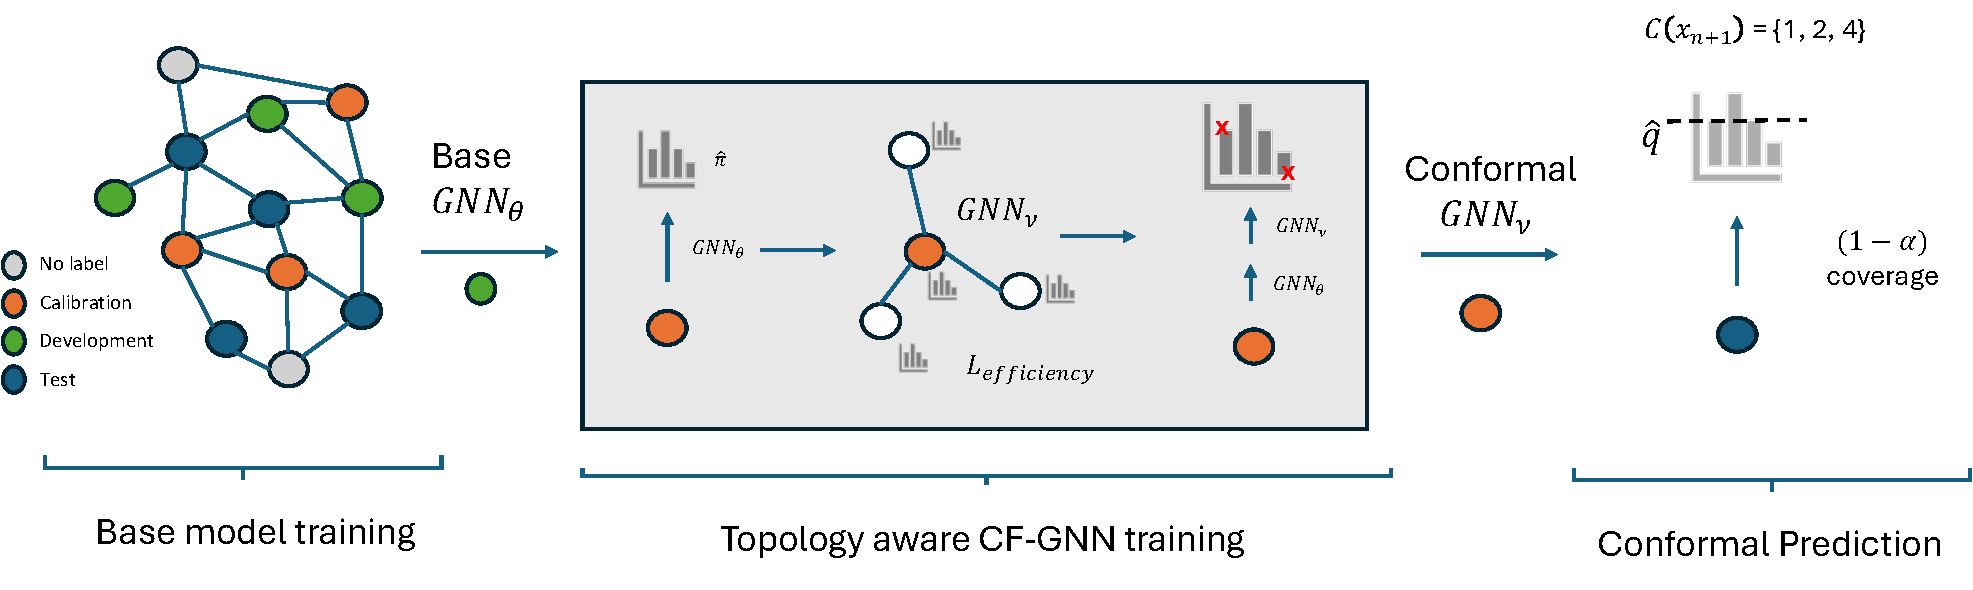
\includegraphics[width=\linewidth]{graphConformal/figures/CFGNN.pdf}
    \caption{Procedure for training CF-GNN. First (left), the base model is trained on the training set. Then, (middle) the CF-GNN is trained to maximize efficiency over the calibration set. Finally , (right) the non-conformity scores from the combined models are used to generate the prediction sets.}
    \label{fig:conformalized_gnn}
\end{figure}

Conformalized GNN (CF-GNN)~\citep{huang2024uncertainty} is a GNN based approach for conformal prediction.
The authors observe that inefficiencies are correlated between nodes having similar neighborhood topology in a graph setting.
They use a GNN during the calibration phase which is trained to correct the scores output from the base model to maximize the efficiency of the conformal prediction.
For classification-based losses, CF-GNN utilizes the fact that all steps in the conformal prediction stage for computing the prediction sets (non-conformity score computation, quantile computation, thresholding) can be expressed as differentiable operations.
Thus, a GNN can be trained directly using efficiency as a loss function.
Figure~\ref{fig:conformalized_gnn} provides a high-level overview of the CF-GNN approach.

\noindent \textbf{CF-GNN Implementation Improvements}
The choice of the conformal loss during calibration and test plays an important role in determining the overall performance of the CF-GNN.
\citet{huang2024uncertainty} use a TPS loss for the calibration phase and the non-randomized APS loss for constructing the final prediction sets.
Our preliminary experiments (Figure~\ref{fig:CFGNN:preliminary}) with replacing the APS loss with a randomized version demonstrated that these losses must be tuned carefully to ensure that the CF-GNN is able to improve upon the base models non-conformity scores.
Some improvements shown in CF-GNN (Figure~\ref{fig:CFGNN:preliminary}, right) get nullified when the randomized APS loss is used (left).
Additionally, CF-GNN uses full batch training which makes it unable to scale for larger graphs.
We implemented a batched version of CF-GNN to ensure that it can be used for larger graphs.
Finally, to speed up computation, we allow the use of cached outputs from the base model rather than having to sample neighbors for both the base model and the CF-GNN. 
This significantly speeds up the computation in both training and evaluation for CF-GNN.

\begin{figure}
    \centering
    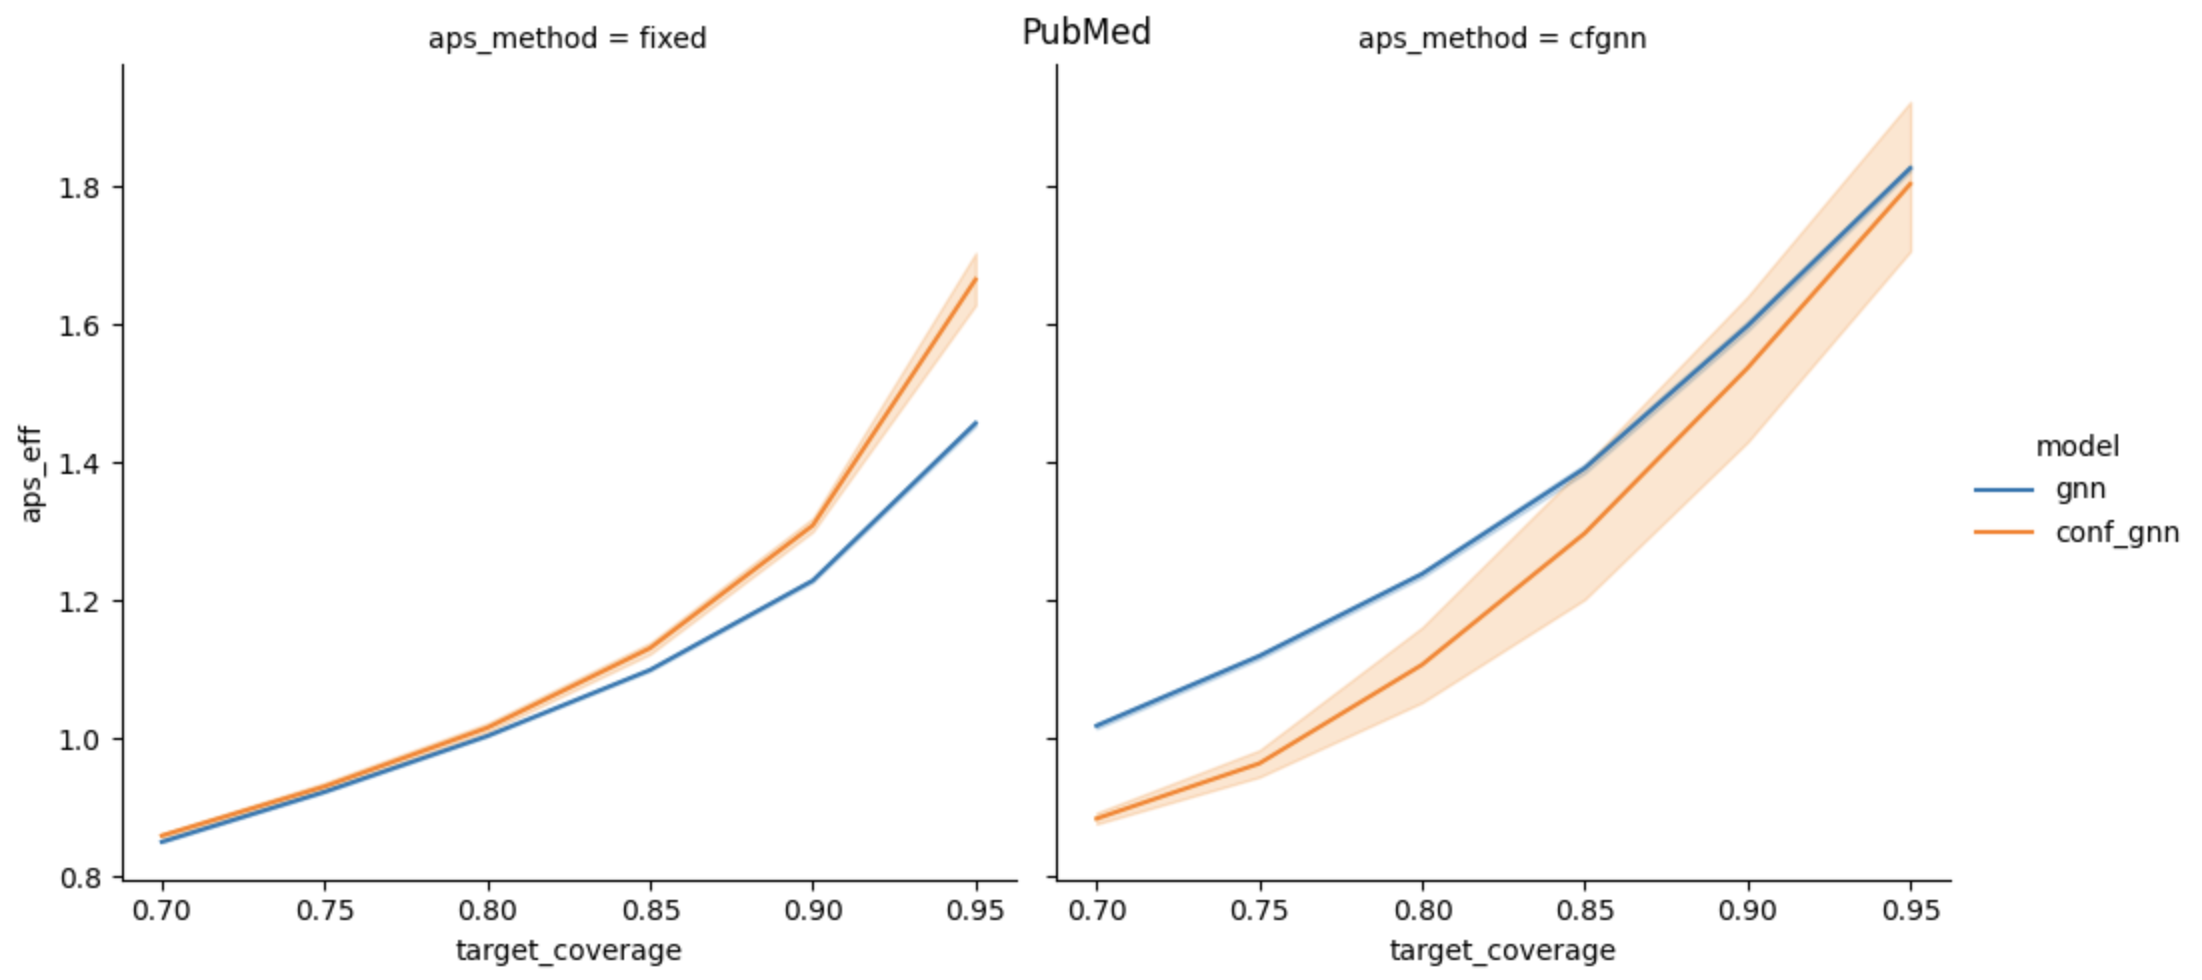
\includegraphics[width=0.8\linewidth]{graphConformal/figures/PubMed_CF.png}
    %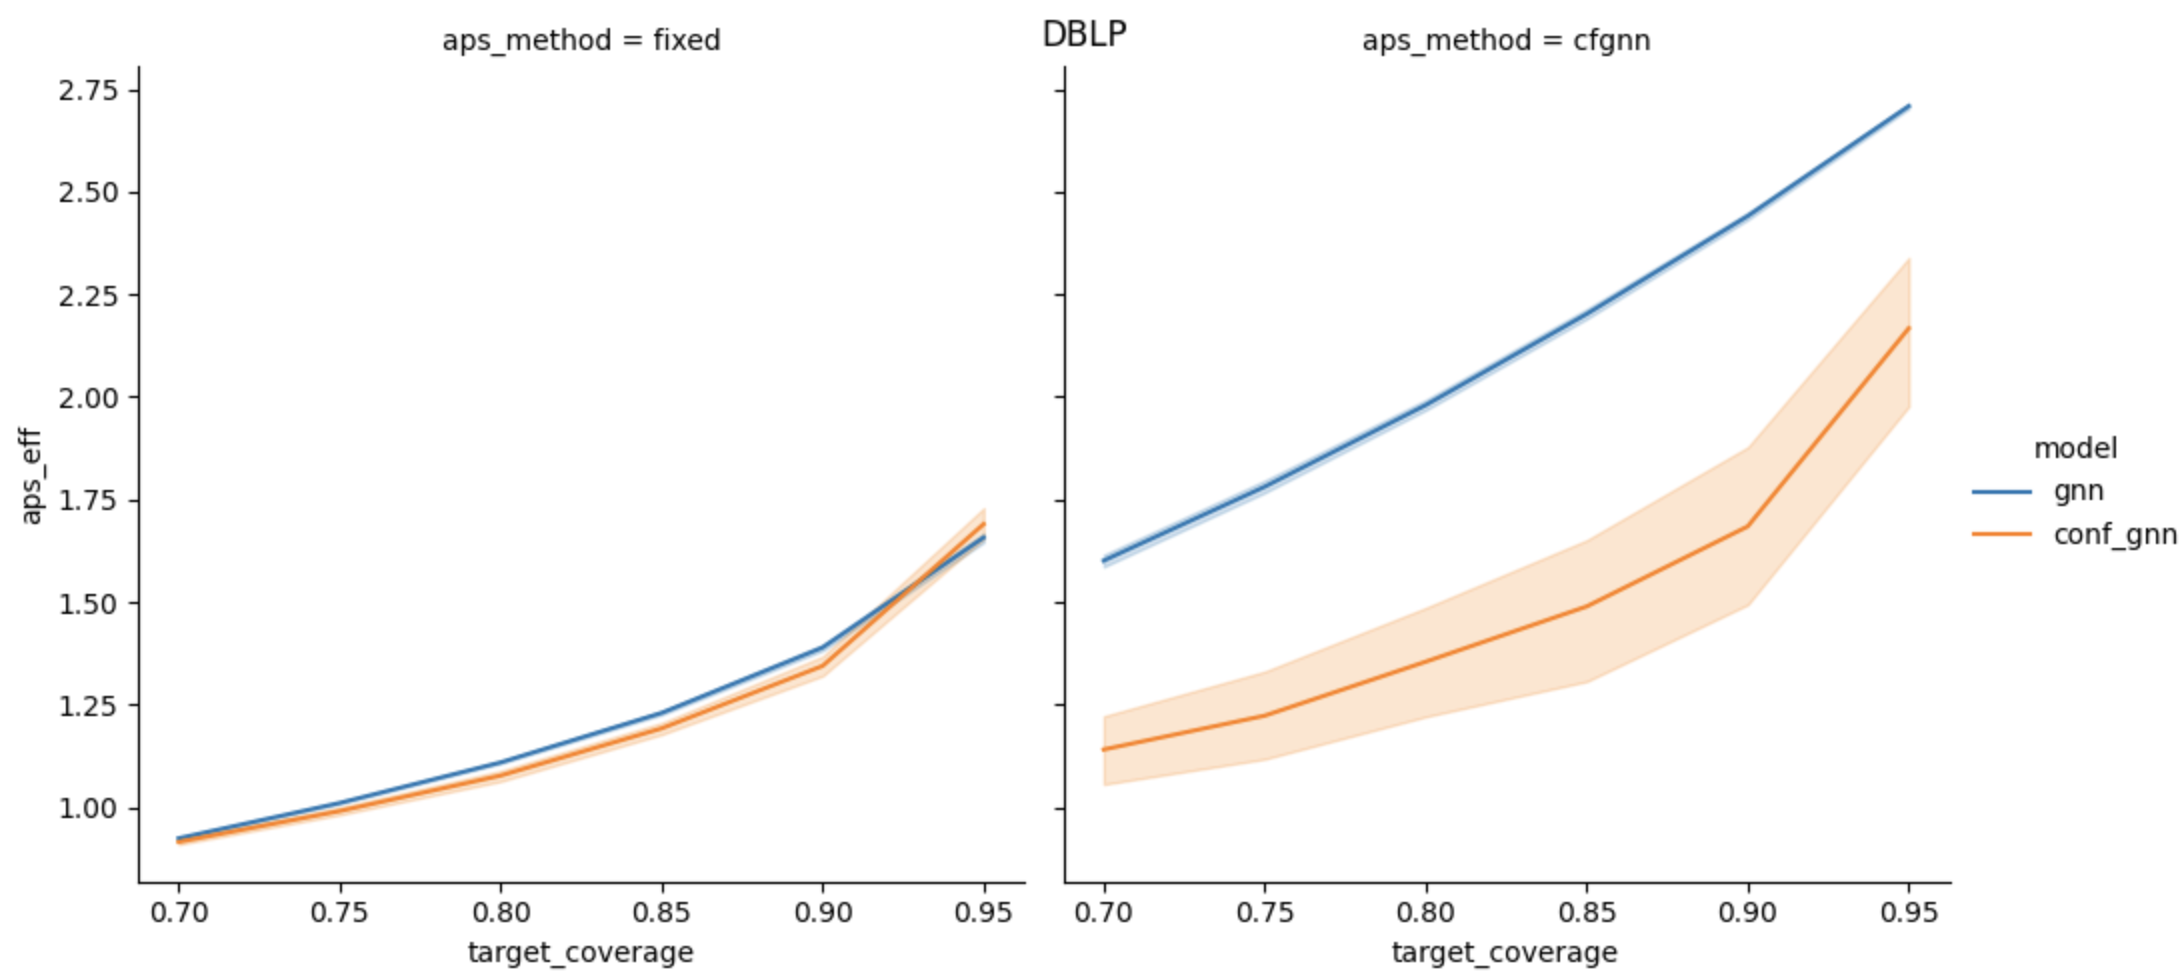
\includegraphics[width=0.7\linewidth]{graphConformal/figures/DBLP_CF.png}
    \caption{Comparing the efficiency (average output set size) for the base model and the CF-GNN on the Pubmed dataset. The plot on the left uses the fixed version of the APS score (with randomized sets) while on the right uses the non-randomized version.}
    \label{fig:CFGNN:preliminary}
\end{figure}
